\chapter{\label{cha:sts_transformers}Adopting Transformers for STS}


Like Recurrent Neural Networks (RNNs), transformers are designed to handle sequential input data, such as natural language, for tasks such as machine translation and text summarisation. However, unlike RNNs, transformers do not necessarily process the data in order. Rather, the attention mechanism provides context for any position in the input sequence. For example, if the input data is a sentence, the transformer does not need to process the beginning of the sentence before the end. 


Transformer models adopt a pre-training followed by fine-tuning scheme which means that once pre-trained these models can be fine-tuned to a large number of down-stream NLP tasks like text classification, named entity recognition etc.  Transformer models, which we have considered in this chapter use special tokens to obtain a single contiguous sequence for each input sequence. Specifically, the first token is always a special classification token \textsc{[CLS]} and sentence pairs are separated using a special token \textsc{[SEP]}. The final hidden state of \textsc{[CLS]}  is used for sentence-level fine-tuning tasks and the final hidden state of each token is used for token-level fine-tuning tasks. The fine-tuning scheme in transformers is usually simple like adding a softmax layer on top of \textsc{[CLS]} token for the text classification tasks. Furthermore, the fine-tuning scheme is very efficient as the parameters in the transformer model are already optimised with the pre-training process. Therefore, transformer models have been extremely popular and successful in many NLP tasks \cite{devlin-etal-2019-bert}. 

In this chapter, we explore different transformers models in variety of STS experiments. 
We address four research questions in this chapter:

\textbf{RQ1:} How well the existing state-of-the-art transformer models perform in STS task? 

\textbf{RQ2:} Can the method further improved with transfer learning and data augmentation techniques?

\textbf{RQ3:} Can the transformer model be easily adopted in to different languages?

\textbf{RQ4:} How well the proposed transformer models perform in a different domain? 

The main contributions of this chapter are as follows.

\begin{enumerate}
\item We evaluate five popular transformer models in three English STS datasets. We compare the results with the previous methods and show that transformer based STS methods outperform all the other STS methods we have experimented.

\item We propose further enhancements to the architecture using inter dataset transfer learning and data augmentation.  

\item We evaluate how well the transformer models perform on STS datasets in different languages and domains. 

\item The code and the pre-trained models are publicly available to the community\footnote{The public GitHub repository is available on \url{https://github.com/tharindudr/STS-Transformers}}. We have published the code as a python library \footnote{The developed python library is available on \url{https://pypi.org/project/ststransformers/}} and by the time of writing this chapter, it has more than 3,000 downloads from the community. 

\end{enumerate}

\section{Related Work}
As we mentioned before, after the introduction of BERT \cite{devlin-etal-2019-bert}, many variants of different transformer models have been proposed by adding minor modifications to the original BERT transformer. Usually these modifications has resulted in improvements in the fine-tuning scheme for the down-stream NLP tasks. Expecting a similar behaviour for the STS task too, we considered following transformer models for the experiments in this chapter.

\paragraph{BERT} \cite{devlin-etal-2019-bert} proposes a masked language modelling (MLM) objective, where some of the tokens of a input sequence are randomly masked, and the objective is to predict these masked positions taking the corrupted sequence as input. BERT applies a Transformer encoder to attend to bi-directional contexts during pre-training. In addition, BERT uses a next-sentence-prediction (NSP) objective. Given two input sentences, NSP predicts whether the second sentence is the actual next sentence of the first sentence. The NSP objective aims to improve the tasks, such as question answering and natural language inference, which require reasoning over sentence pairs. 

\paragraph{RoBERTa} \cite{liu2019roberta} makes a few changes to the BERT architecture and achieves substantial improvements. The changes include: (1) Training the model longer with larger batches and more data; (2) Removing the NSP objective; (3) Training on longer sequences; (4) Dynamically changing the masked positions during pre-training.

\paragraph{ALBERT} \cite{Lan2020ALBERT} proposes two parameter-reduction techniques (factorised embedding parameterisation and cross-layer parameter sharing) to lower memory consumption and speed up training. Furthermore, ALBERT \cite{Lan2020ALBERT} argues that the NSP objective in BERT lacks difficulty, as the negative examples are created by pairing segments from different documents, this mixes topic prediction and coherence prediction into a single task. ALBERT instead uses a sentence-order prediction
(SOP) objective. SOP obtains positive examples by taking out two consecutive segments and negative examples by reversing the order of two consecutive segments from the same document.


\paragraph{ELECTRA} Compared to BERT, ELECTRA \cite{Clark2020ELECTRA} proposes a more effective pre-training method. Instead of corrupting some positions of inputs with [MASK], ELECTRA replaces some tokens of the inputs with their plausible alternatives sampled from a small generator network. ELECTRA trains a discriminator to predict whether each token in the corrupted input was replaced by the generator or not. The pre-trained discriminator can then be used in downstream tasks for fine-tuning, improving upon the pre-trained representation learned by the generator.

\paragraph{XLNET} \cite{yang2019xlnet} identifies a key weakness in BERT pre-training. \citet{yang2019xlnet} argues that the symbols such as \textsc{[MASK]} that are introduced by BERT during pre-training, causes discrepancy between pre-training and fine-tuning as they never occur in real data. Therefore, XLNET suggests a new auto-regressive method based on permutation language modelling (PLM) \cite{JMLR:v17:16-272} without introducing any new symbols. 

Upon the introduction all of these transformer models have been evaluated in many down-stream NLP tasks including STS too. However, there is no comprehensive study done on STS using transformers considering big and small datasets, transfer learning, data augmentation, multilingual STS etc. which we do in this chapter.

\section{Transformer Architecture for STS}

The transformer architecture for STS is shown in Figure \ref{fig:sts_transformers}. The input of this model is a concatenation of the two sentences, separated by the \textsc{[SEP]} token. Then the output of the \textsc{[CLS]} token is used as the input of a softmax layer that predicts the similarity of the two sentences. We used mean-squared-error loss as the objective function. As the configurations, we used a batch-size of eight, Adam optimiser with learning rate $2\mathrm{e}{-5}$, and a linear learning rate warm-up over 10\% of the training data. During the training process, the parameters of the transformer, as well as the parameters of the subsequent layers, were updated. The models were trained using only training data. Furthermore, they were evaluated while training after each 100 batches, using an evaluation set that had one fifth of the rows in training data. We performed early stopping if the evaluation loss did not improve over ten evaluation steps. All the models were trained for three epochs. As these transformer models are computationally expensive, we used an Nvidia Tesla T4 GPU for the training process. We have kept these configuration same for all the experiments; in order to ensure consistency between all the languages and domains. This also provides a good starting configuration for researchers who intend to use transformers on a new language pair. The implementation is based on PyTorch \cite{NEURIPS2019_9015} and HuggingFace \cite{wolf-etal-2020-transformers}.

\begin{figure}[ht]
	\centering
	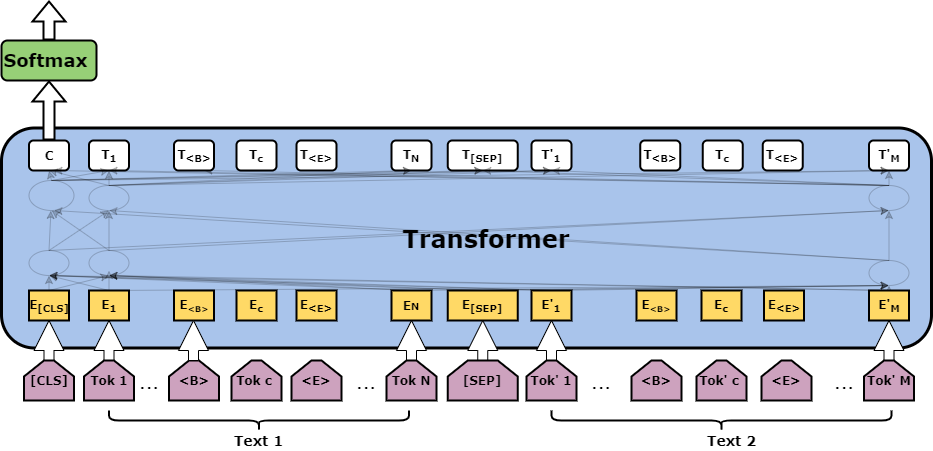
\includegraphics[scale=0.4]{figures/semantic_textual_similarity/transformers/STSTransformers.png}
	\caption[Architecture for using Transformers in STS]{Architecture for using Transformers in STS.}
	\label{fig:sts_transformers}
\end{figure}

\section{Exploring Transformers in English STS}
We evaluated all the above transformer variations in the three English STS datasets we introduced in \ref{cha:sts_introduction}; SICK, STS 2017 and QUORA. All of the transformer models we considered have several models that supports English (e.g.\ \textit{bert-large-cased} \& \textit{bert-base-cased} for BERT, \textit{albert-xxlarge-v2} \& \textit{albert-base-v2} for ALBERT) and usually the large models outperform the smaller models in downstream tasks. Therefore, we used the largest possible model that our GPU setup can load with each transformer type; \textit{bert-large-cased} for BERT \cite{devlin-etal-2019-bert}, \textit{albert-large-v2} for ALBERT \cite{Lan2020ALBERT}, \textit{roberta-large} for RoBERTa \cite{liu2019roberta}, \textit{google/electra-large-discriminator} for ELECTRA \cite{Clark2020ELECTRA} and \textit{xlnet-large-cased}  \cite{yang2019xlnet} for XLNET. All of these models are available in HuggingFace \cite{wolf-etal-2020-transformers} model hub\footnote{Models are available on \url{https://huggingface.co/models}}.

We trained the transformer models on the training sets on those datasets and evaluated them on the testing sets. The results are shown in Table \ref{tab:sick_transformers}, Table \ref{tab:sts_transformers} and Table \ref{tab:quora_transformers} respectively. 

\begin{table*}[htb]
	%\footnotesize
	\centering
	\scalebox{0.95}{
		\begin{tabular}{|l|cc|}
			\hline
			\textbf{Model} & $\bm{\rho}$   & $\bm{\tau}$     
			\\ \hline
			\textit{BERT}                  
			& 0.881 & 0.826  \\
			\textit{ALBERT}                  
			& 0.886 & 0.829  \\
			\textit{RoBERTa}                  
			& 0.892$^{\dagger}$ & 0.834$^{\dagger}$  \\
			\textit{ELECTRA}                  
			& 0.872 & 0.819  \\
			\textit{XLNET}                  
			& 0.879 & 0.821  \\
			\hline
		\end{tabular}
	}
	\caption[Results for SICK with Transformer Models]{Results for SICK dataset with different variants of transformer models. For each variant, Pearson Correlation ($\bm{\rho}$) and Spearman Correlation ($\bm{\tau}$) are reported between the predicted values and the gold labels of the test set. Best result from all the variations is marked with ${\dagger}$.}  
	\label{tab:sick_transformers}
\end{table*}


\begin{table*}[htb]
	%\footnotesize
	\centering
	\scalebox{0.95}{
		\begin{tabular}{|l|cc|}
			\hline
			\textbf{Model} & $\bm{\rho}$   & $\bm{\tau}$     
			\\ \hline
				\textit{BERT}                  
		& 0.889 & 0.858  \\
		\textit{ALBERT}                  
		& 0.874 & 0.852  \\
		\textit{RoBERTa}                  
		& 0.895$^{\dagger}$ & 0.861$^{\dagger}$  \\
		\textit{ELECTRA}                  
		& 0.873 & 0.849  \\
		\textit{XLNET}                  
		& 0.868 & 0.843  \\
			\hline
		\end{tabular}
	}
	\caption[Results for STS 2017 with Transformers]{Results for STS 2017 dataset with different variants of Transformers. For each variant, Pearson Correlation ($\bm{\rho}$) and Spearman Correlation ($\bm{\tau}$) are reported between the predicted values and the gold labels of the test set. Best result from all the variations is marked with ${\dagger}$. }  
	\label{tab:sts_transformers}
\end{table*}


\begin{table*}[htb]
	%\footnotesize
	\centering
	\scalebox{0.95}{
		\begin{tabular}{|l|c|}
			\hline
			\textbf{Model} & RMSE     
			\\ \hline
			\textit{BERT}                  
			& 0.349   \\
			\textit{ALBERT}                  
			& 0.354   \\
			\textit{RoBERTa}                  
			& 0.359   \\
			\textit{ELECTRA}                  
			& 0.353   \\
			\textit{XLNET}                  
			& 0.346$^{\dagger}$   \\
			\hline
		\end{tabular}
	}
	\caption[Results for QUORA with Transformers]{Results for QUORA dataset with different variants of Transformers. For each variant, Root Mean Squared Error (RMSE) reported between the predicted values and the gold labels of the test set. Best result from all the variations is marked with ${\dagger}$. }  
	\label{tab:quora_transformers}
\end{table*}

As can be seen in Table \ref{tab:sick_transformers} and \ref{tab:sts_transformers}, for SICK and STS 2017 datasets, RoBERTa outperformed other transformer models. Since SICK and STS 2017 are smaller datasets, optimised nature in RoBERTa seems to be beneficial in smaller datasets. In the QUORA dataset, which is considerably bigger than SICK and STS 2017, \textit{XLNET}  outperforms other transformer models. However, from the results, there is no clear indication that which transformer model would perform best in a certain dataset other than the fact that 	\textit{RoBERTa} performs slightly better in smaller datasets. It should be noted that, all of the transformers perform on par with each other. 

In the initial experiments, we noticed that the transformer models are quite sensitive to the random seed\footnote{Random seed id used to configure the starting weights in a neural network. Keeping the random seed constant from one experiment to the next removes the variation due to this randomness, making it easier to interpret the effects of other design changes such as hyper parameter values.} of the experiments \cite{zhang2021revisiting}. Changing the random seed led to very different results. To minimise this affect from random seed, we conducted the experiments for five different random seeds and took the mean of these experiments as the final results which is the value reported in Tables \ref{tab:sick_transformers}, \ref{tab:sts_transformers} and \ref{tab:quora_transformers}. We noticed that doing many experiments with different random seeds reduced the variance of the final result. 

With this we answer our \textbf{RQ1}: transformers can be successful adopted in the STS task and they produce good results in all the datasets. For the smaller datasets, \textit{RoBERTa} performed slightly better than other transformer models. Furthermore, we recommend to conduct more experiments with different random seeds in order to minimise the variance.


\subsection{Impact of Transfer Learning}
Similar to the \textit{Siamese neural networks} in Chapter \ref{cha:sts_siamese_neural_networks}, we explored the impact of transfer learning  in STS, with transformers too. We saved the weights of the transformers models that were trained on each STS dataset; SICK, STS 2017 and QUORA. We specifically used the two models that performed best in these dataset; RoberTa and XLNET. We again initiated training for each dataset, however rather than training the transformer model from scratch, we used the weights of the models trained on other STS dataset. We compared this transfer learning results to the results we got from training the model from scratch. Similar to the \textit{Siamese neural network} experiments, we conducted this transfer learning experiment only on STS2017 and SICK dataset since the QUORA dataset was already big and transfer learning from a smaller dataset to a larger dataset won't make much sense.


\begin{table*}[htb]
	%\footnotesize
	\centering
	\scalebox{0.95}{
		\begin{tabular}{|l|c|c|}
			\hline
			\textbf{Start Model} & STS2017 & SICK      
			\\ \hline
			\textit{STS2017$_{RoBERTa}$}                  
			& 0.853 & \textcolor{gray}{(+0.009)} \\
			\textit{STS2017$_{XLNET}$}                     
			& 0.830 & \textcolor{gray}{(+0.011)}  \\
			\hline
			\textit{SICK$_{RoBERTa}$}                     
			& \textcolor{gray}{(+0.008)} & 0.838 \\
			\textit{SICK$_{XLNET}$}                     
			& \textcolor{gray}{(+0.013)} & 0.827 \\
			\hline
			\textit{QUORA$_{RoBERTa}$}                     
			& \textcolor{gray}{(-0.025)}  &  \textcolor{gray}{(-0.021)}    \\
			\textit{QUORA$_{XLNET}$}                     
			& \textcolor{gray}{(-0.039)} &  \textcolor{gray}{(-0.043)}    \\
			\hline
		\end{tabular}
	}
	\caption[Results for transfer learning with Transformers]{Results for transfer learning with different Transformers. For each transfer learning experiment we show the difference between with transfer learning and without transfer learning. Non-grey values are the results of the experiments without transfer learning which we showed in the previous section too. We only report the Pearson correlation due to ease of visualisation.}  
	\label{tab:transfer_transformers}
\end{table*}



\subsection{Impact of Data Augmentation}

\begin{table*}[htb]
	%\footnotesize
	\centering
	\scalebox{0.95}{
		\begin{tabular}{|c|c|c|}
			\hline
			\textbf{Dataset} &	\textbf{Start Model} &  $\bm{\rho}$      
			\\ \hline
			\multirow{ 2}{*}{\textit{SICK}}	& \textit{STS2017$_{RoBERTa}$}                  
			& \textcolor{gray}{(+0.01)} \\
			&	\textit{STS2017$_{XLNET}$}                     
			& \textcolor{gray}{(+0.01)}  \\
			\hline
			\multirow{ 2}{*}{\textit{STS2017}}  & \textit{SICK$_{RoBERTa}$}                     
			& \textcolor{gray}{(+0.01)}  \\
			& \textit{SICK$_{XLNET}$}                     
			& \textcolor{gray}{(+0.01)} \\
			\hline
		\end{tabular}
	}
	\caption[Results for data augmentation with Transformers]{Results for data augmentation with different Transformers. For each data augmentation experiment we show the difference between with dat augmentation and without data augmentation. We only report the Pearson correlation ($\bm{\rho}$) due to ease of visualisation.}  
	\label{tab:augmentation_transformers}
\end{table*}



\begin{table*}[htb]
	%\footnotesize
	\centering
	\scalebox{0.95}{
		\begin{tabular}{|l|c|}
			\hline
			\textbf{Model} & $\bm{\rho}$      
			\\ \hline
			\citet{jimenez-etal-2014-unal} & 0.807 \\
			\citet{bjerva-etal-2014-meaning} & 0.827 \\
			\citet{zhao-etal-2014-ecnu-one} & 0.841 \\
			\textit{Siamese LSTM} & 0.863  \\
			\textit{Siamese GRU} & 0.882  \\
			\hline
		\end{tabular}
	}
	\caption[Results comparison for SICK with leader board results]{Results for SICK dataset with different transformer models. For each variant, Pearson Correlation ($\bm{\rho}$) is reported between the predicted values and the gold labels of the test set.}  
	\label{tab:sick_transformers_all}
\end{table*}

\begin{table*}[htb]
	%\footnotesize
	\centering
	\scalebox{0.95}{
		\begin{tabular}{|l|c|}
			\hline
			\textbf{Model} & $\bm{\rho}$      
			\\ \hline
			\citet{tian-etal-2017-ecnu} & 0.851 \\
			\textit{Siamese LSTM} & 0.852  \\
			\citet{maharjan-etal-2017-dt} & 0.854 \\
			\citet{cer-etal-2017-semeval}  & 0.855   \\
			\textit{Siamese GRU} & 0.862  \\
			\hline
		\end{tabular}
	}
	\caption[Results comparison for STS2017 with leader board results]{Results for STS2017 dataset with different variants of Siamese Neural Network. For each variant, Pearson Correlation ($\bm{\rho}$) is reported between the predicted values and the gold labels of the test set.  }  
	\label{tab:sts_transformers_all}
\end{table*}

\section{Portability to Other Languages}

\begin{table*}[htb]
	%\footnotesize
	\centering
	\scalebox{0.95}{
		\begin{tabular}{|l|cc|}
			\hline
			\textbf{Model} & $\bm{\rho}$   & $\bm{\tau}$     
			\\ \hline
			\textit{LSTM}                  
			& 0.746 & 0.690  \\
			\textit{Bi-LSTM}                     
			& 0.725 & 0.683   \\
			\textit{GRU}                     
			& 0.763$^{\dagger}$ & 0.723$^{\dagger}$  \\
			\textit{Bi-GRU}                     
			& 0.752 & 0.717  \\
			\textit{LSTM + Attention}                     
			& 0.741  & 0.703       \\
			\textit{GRU + Attention}                     
			& 0.739  & 0.691       \\
			\textit{GRU + Capsule + Flatten}                     
			& 0.712  & 0.679       \\
			\hline
		\end{tabular}
	}
	\caption[Results for Arabic STS with Transformers]{Results for Arabic STS dataset with different transformers. For each variant, Pearson Correlation ($\bm{\rho}$) and Spearman Correlation ($\bm{\tau}$) are reported between the predicted values and the gold labels of the test set. Best result from all the variations is marked with ${\dagger}$. }  
	\label{tab:arabic_transformers}
\end{table*}


\begin{table*}[htb]
	%\footnotesize
	\centering
	\scalebox{0.95}{
		\begin{tabular}{|l|cc|}
			\hline
			\textbf{Model} & $\bm{\rho}$   & $\bm{\tau}$     
			\\ \hline
			\textit{LSTM}                  
			& 0.842 & 0.773  \\
			\textit{Bi-LSTM}                     
			& 0.814 & 0.782   \\
			\textit{GRU}                     
			& 0.863$^{\dagger}$ & 0.822$^{\dagger}$  \\
			\textit{Bi-GRU}                     
			& 0.851 & 0.813  \\
			\textit{LSTM + Attention}                     
			& 0.845  & 0.801       \\
			\textit{GRU + Attention}                     
			& 0.832  & 0.790       \\
			\textit{GRU + Capsule + Flatten}                     
			& 0.795  & 0.773       \\
			\hline
		\end{tabular}
	}
	\caption[Results for Spanish STS with Transformers]{Results for Spanish STS dataset with different Transformers. For each variant, Pearson Correlation ($\bm{\rho}$) and Spearman Correlation ($\bm{\tau}$) are reported between the predicted values and the gold labels of the test set. Best result from all the variations is marked with ${\dagger}$. }  
	\label{tab:spanish_transformers}
\end{table*}

Furthermore, we compared the results of the best transformer model with the best results submitted to the competition \cite{cer-etal-2017-semeval} and with the supervised/unsupervised STS methods we have experimented so far in this part of the thesis. 


\begin{table*}[htb]
	%\footnotesize
	\centering
	\scalebox{0.95}{
		\begin{tabular}{|l|c|}
			\hline
			\textbf{Model} & $\bm{\rho}$      
			\\ \hline
			\citet{tian-etal-2017-ecnu} & 0.744 \\
			\citet{nagoudi-etal-2017-lim} & 0.746 \\
			\textit{Siamese LSTM} & 0.746  \\
			\citet{wu-etal-2017-bit}  & 0.754   \\
			\textit{Siamese GRU} & 0.763  \\
			\hline
		\end{tabular}
	}
	\caption[Results comparison for Arabic STS with leader board results]{Results for Arabic STS dataset with different transformers. For each variant, Pearson Correlation ($\bm{\rho}$) is reported between the predicted values and the gold labels of the test set.  }  
	\label{tab:arabic_transformers_all}
\end{table*}


\begin{table*}[htb]
	%\footnotesize
	\centering
	\scalebox{0.95}{
		\begin{tabular}{|l|c|}
			\hline
			\textbf{Model} & $\bm{\rho}$   \\  
			\hline
			\textit{Siamese LSTM} & 0.842  \\
			\citet{hassan-etal-2017-fcicu} & 0.848 \\
			\citet{wu-etal-2017-bit} &  0.850 \\
			\citet{tian-etal-2017-ecnu} & 0.855 \\
			\textit{Siamese GRU} & 0.863  \\
			\hline
		\end{tabular}
	}
	\caption[Results comparison for Spanish STS with leader board results]{Results for Spanish STS dataset with different variants of Siamese Neural Network. For each variant, Pearson Correlation ($\bm{\rho}$) is reported between the predicted values and the gold labels of the test set. }  
	\label{tab:spanish_transformers_all}
\end{table*}


\section{Potability to Other Domains}

\begin{table*}[htb]
	%\footnotesize
	\centering
	\scalebox{0.95}{
		\begin{tabular}{|l|c|c|}
			\hline
			\textbf{Model} & Word2vec & BioWordVec      
			\\ \hline
			\textit{STS2017$_{GRU}$}                  
			& 0.651 & 0.721 \\
			\textit{STS2017$_{LSTM+Aten}$}                     
			& 0.612 & 0.701  \\
			\hline
			\textit{SICK$_{GRU}$}                     
			& 0.642 & 0.719 \\
			\textit{SICK$_{LSTM+Aten}$}                     
			& 0.608 & 0.699 \\
			\hline
			\textit{QUORA$_{GRU}$}                     
			& 0.591  &  0.622    \\
			\textit{QUORA$_{LSTM+Aten}$}                     
			& 0.603 &  0.634   \\
			\hline
		\end{tabular}
	}
	\caption[Results for transfer learning with Siamese Neural Network in BIOSSES dataset]{Results for transfer learning with different variants of Siamese Neural Network in BIOSSES dataset. Two considered word embedding models are Word2vec and BioWordVec. We only report the Pearson correlation due to ease of visualisation.}  
	\label{tab:transfer_transformers_biosses}
\end{table*}

\begin{table*}[htb]
	%\footnotesize
	\centering
	\scalebox{0.95}{
		\begin{tabular}{|l|c|}
			\hline
			\textbf{Model} & $\bm{\rho}$   \\  
			\hline
			\textit{ELMo $\bigoplus$ BERT}  &  0.708 \\
			\textit{STS2017$_{GRU}$} & 0.719 \\
			\citet{10.1093/bioinformatics/btx238} & 0.754 \\
			\textit{BioSentVec} \cite{8904728} & 0.810  \\
			\hline
		\end{tabular}
	}
	\caption[Results comparison for BIOSSES with top results]{Results for BIOSSES dataset with different variants of Siamese Neural Network compared with top results reported for BIOSSES. For each variant, Pearson Correlation ($\bm{\rho}$) is reported between the predicted values and the gold labels of the test set. }  
	\label{tab:biosses_transformers_all}
\end{table*}

\section{Recent Developments: Siamese Transformers}

\section{Conclusions}